\PassOptionsToPackage{xetex}{xcolor}
\PassOptionsToPackage{xetex}{graphicx}
\documentclass[a4paper,landscape,headrule,footrule,xetex]{foils}

%%
%%%  Macros
%%%
\newcommand{\logo}{~}
\MyLogo{HG2052 (2020)}
%\newcommand{\Story}{\SHA{HOUN}{The Hound of the Baskervilles}}

\newcommand{\header}[3]{%
\title{\vspace*{-2ex} \Large HG2052
\\\large  Language, Technology and the Internet
\\[2ex] \Large  \emp{#2}}
\author{\blu{Francis Bond}   \\ 
\normalsize  \textbf{Division of Linguistics and Multilingual Studies}\\
\normalsize  \url{http://www3.ntu.edu.sg/home/fcbond/}\\
\normalsize  \texttt{bond@ieee.org}}
\MyLogo{HG2052 (2020)}
\date{#1}
\renewcommand{\logo}{#2}
 \hypersetup{
   pdfinfo={
     Author={Francis Bond},
     Title={#1: #2},
     Subject={HG2052: Language, Technology and the Internet},
     Keywords={Language, Technology, Internet},
     License={CC BY 4.0}
   }
 %  pdfcopyright={Copyright © Francis Bond. Creative Commons 4.0 Attribution License.}
 %  pdflicenseurl={http://creativecommons.org/licenses/by/4.0/}
 }
}


%%
%% Multilingual Stuff
%%
\usepackage[a4paper,landscape,margin=25mm]{geometry}

\usepackage{fontenc}
\usepackage{polyglossia}
\setmainlanguage{english}
\setmainfont{TeX Gyre Pagella}
%\setmainfont{Linux Libertine}
%\setmainfont{Charis SIL}
\newfontfamily{\ipafont}{Gentium}
\newcommand{\ipa}[1]{{\ipafont\selectfont #1}}
\usepackage{xeCJK}

\setCJKmainfont{Noto Sans CJK SC}
\setCJKsansfont{Noto Sans CJK SC}
%\setCJKttfont{Noto Sans CJK SC}
%\setCJKmainfont{WenQuanYi Micro Hei}
%\clearpage
%\setCJKmainfont{AR PL SungtiL GB}

\usepackage[xetex]{xcolor}
\usepackage[xetex]{graphicx}
\newcommand{\blu}[1]{\textcolor{blue}{#1}}
\newcommand{\grn}[1]{\textcolor{green}{#1}}
\newcommand{\hide}[1]{\textcolor{white}{#1}}
\newcommand{\emp}[1]{\textcolor{red}{#1}}
\newcommand{\txx}[1]{\textbf{\textcolor{blue}{#1}}}
\newcommand{\lex}[1]{\textbf{\mtcitestyle{#1}}}

\usepackage{pifont}
\renewcommand{\labelitemi}{\textcolor{violet}{\ding{227}}}
\renewcommand{\labelitemii}{\textcolor{purple}{\ding{226}}}

\newcommand{\subhead}[1]{\noindent\textbf{#1}\\[5mm]}

\newcommand{\Bad}{\emp{\raisebox{0.15ex}{\ensuremath{\mathbf{\otimes}}}}}
\newcommand{\bad}{*}

\newcommand{\com}[1]{\hfill \textnormal{(\emp{#1})}}%
\newcommand{\cxm}[1]{\hfill \textnormal{(\txx{#1})}}%
\newcommand{\cmm}[1]{\hfill \textnormal{(#1)}}%
\usepackage{amssymb}
\usepackage{relsize,xspace}
\newcommand{\into}{\ensuremath{\rightarrow}\xspace}
\newcommand{\ent}{\ensuremath{\Rightarrow}\xspace}
\newcommand{\nent}{\ensuremath{\not\Rightarrow}\xspace}
\newcommand{\tot}{\ensuremath{\leftrightarrow}\xspace}
\usepackage{url}
\usepackage[hidelinks]{hyperref}
\hypersetup{
     colorlinks,
     linkcolor={blue!50!black},
     citecolor={red!50!black},
     urlcolor={blue!80!black}
}
%\usepackage{hyperxmp}
\usepackage{url}
\newcommand{\lurl}[1]{\MyLogo{\url{#1}}}

\usepackage{mygb4e}
\let\eachwordone=\itshape
\newcommand{\lx}[1]{\textbf{\textit{#1}}}
\newcommand{\ix}{\ex\it}

\newcommand{\cen}[2]{\multicolumn{#1}{c}{#2}}
%\usepackage{times}
%\usepackage{nttfoilhead}
\newcommand{\myslide}[1]{%
\foilhead[-25mm]{\raisebox{12mm}[0mm]{\emp{#1}}}%
\leftheader{}%
\MyLogo{\logo}}

\newcommand{\mytask}[1]{%
\foilhead[-25mm]{\raisebox{12mm}[0mm]{\emp{#1}}}
\leftheader{🔍 Hi}%
\MyLogo{\logo}}

\newcommand{\myslider}[1]{\rotatefoilhead[-25mm]{\raisebox{12mm}[0mm]{\emp{#1}}}}
%\newcommand{\myslider}[1]{\rotatefoilhead{\raisebox{-8mm}{\emp{#1}}}}

\newcommand{\section}[1]{\myslide{}{\begin{center}\Huge \emp{#1}\end{center}}}

\usepackage{tcolorbox}
% \newcommand{\task}{\marginpar{\raisebox{-1ex}{\large
%       \tcbox[colframe=red,colback=white,arc=3pt]{\textbf{?}}}}}
% \newcommand{\task}{\marginpar{\raisebox{-1ex}{
%       \hspace{-0.5em}\tcbox[colframe=red,colback=white,arc=3pt]{%
%         \includegraphics[width=1.5em]{pics/detective}}}}}
\newcommand{\task}{\marginpar{\raisebox{-2ex}{
      \hspace{-0.5em}\reflectbox{\includegraphics[width=2em]{pics/detective}}}}}

\usepackage[lyons,j,e,k]{mtg2e}
\renewcommand{\mtcitestyle}[1]{\textcolor{teal}{\textsl{#1}}}
%\renewcommand{\mtcitestyle}[1]{\textsl{#1}}
\newcommand{\chn}{\mtciteform}
\newcommand{\cmn}{\mtciteform}
\newcommand{\iz}[1]{\textup{\texttt{\textcolor{blue}{\textbf{#1}}}}}
\newcommand{\con}[1]{\textsc{#1}}
\newcommand{\gm}{\textsc}
\newcommand{\cmp}[1]{{[\textsc{#1}]}}
\newcommand{\sr}[1]{\ensuremath{\langle}#1\ensuremath{\rangle}}
\usepackage[normalem]{ulem}
\newcommand{\ul}{\uline}
\newcommand{\uul}{\uuline}
\newcommand{\wl}{\uwave}
\newcommand{\vs}{\ensuremath{\Leftrightarrow}~}
%%%
%%% Bibliography
%%%
\usepackage{natbib}
%\usepackage{url}
\usepackage{bibentry}


%%% From Tim
\newcommand{\WMngram}[1][]{$n$-gram#1\xspace}
\newcommand{\infers}{$\rightarrow$\xspace}



\usepackage{rtrees,qtree}
\renewcommand{\lf}[1]{\br{#1}{}}
\usepackage{avm}
%\avmoptions{topleft,center}
\newcommand{\ft}[1]{\textsc{#1}}
\newcommand{\val}[1]{\textit{#1}}
\newcommand{\typ}[1]{\textit{#1}}
\avmfont{\sc}
%\avmvalfont{\sc}
\renewcommand{\avmtreefont}{\sc}
\avmsortfont{\it}


%%% From CSLI book
\newcommand{\mc}{\multicolumn}
\newcommand{\HD}{\textbf{H}\xspace}
\newcommand{\el}{\< \>}
\makeatother
\long\def\smalltree#1{\leavevmode{\def\\{\cr\noalign{\vskip12pt}}%
\def\mc##1##2{\multispan{##1}{\hfil##2\hfil}}%
\tabskip=1em%
\hbox{\vtop{\halign{&\hfil##\hfil\cr
#1\crcr}}}}}
\makeatletter

\newcommand{\sh}[1]{\href{https://www.arthur-conan-doyle.com/index.php?title=#1}{#1}}
\newcommand{\SHA}[2]{\href{https://www.arthur-conan-doyle.com/index.php?title=#1}{\textit{#2}}}


\header{Lecture 1}{Introduction, Organization: Overview,  Main Issues}

\usepackage{qtree}
\newcommand{\clsiz}[2]{%
\begin{tabular}{c}%
\iz{#1}\\ (#2)%
\end{tabular}%
}
\newcommand{\cljpn}[2]{%
\makebox[0mm][r]{\begin{tabular}[t]{c}%
\textsl{#1}\\ {\small ``#2''}%
\end{tabular}}%
}
\newcommand{\sss}[1]{\makebox[0mm][r]{\textsl{#1}}}

% \usepackage{mygb4e}
% \newcommand{\refs}[1]{(\ref{s:#1})}
% \newcommand{\exs}[1]{\ex\label{s:#1}}
% \singlegloss


\begin{document}

\maketitle


\myslide{Introduction}

\begin{itemize}
\item How technology affects our use of language
% (from the effects of encoding to the rise of chatspeak), and also
 \item How language is used on the internet
   \begin{itemize}
   \item Some fun things we can now do, that we couldn't before 
   \end{itemize}
 \item Collaboration and shared authoring
 \item Meta-languages
 \item The Semantic Web
%   Students will gain understanding of the 
% problems of representing, transmitting and transforming language
% electronically.  Specific topics will include automatic parsing and
% generation of language, text mining (extracting knowledge from text)
% and machine translation.
\end{itemize}


\myslide{Goals}
\begin{itemize}
\item Gain an understanding of how technology affects language use
\item Develop familiarity with markup and meta information in texts
\item Get a feel for what research is all about, especially relating to
  web mining and online frequency counting
\end{itemize}
\subhead{Upon successful completion, students will:}
\begin{itemize}
\item have an understanding of how technology shapes language use
\item be able to test linguistic hypotheses against web data.
\end{itemize}



% \myslide{Personal Introduction}

% \begin{itemize}\addtolength{\itemsep}{-0.5ex}
% %\item Francis Bond 
% \item BA in Japanese and Mathematics 
% \item BEng in Power and Control %(Electrical Systems Engineering)
%   \hspace{7em}\raisebox{0ex}[0mm][0mm]{\includegraphics{pwm.eps}}
% \item PhD on  ``Determiners and Number in English
%   contrasted with Japanese,  as exemplified in Machine
%   Translation'' 
% \item 1991-2006 NTT (Nippon Telegraph and Telephone)
%   \begin{itemize}%\addtolength{\itemsep}{-0.5ex}
%   \item Japanese - English/Malay Machine Translation
%   \item Japanese corpus, grammar and ontology (Hinoki)
%   \end{itemize}
% \item 2006-2009 NICT (National Inst. for Info. and Comm. Technology)
%   \begin{itemize}%\addtolength{\itemsep}{-0.5ex}
%   \item Japanese - English, Chinese Machine Translation
%   \item Japanese WordNet
%   \end{itemize}
% %\item 2009- NTU
% \end{itemize}

\myslide{Administrivia}

\begin{description}
\item [Coordinator]  Francis \ul{Bond}
\item [Email] \url{bond@ieee.org}; \textbf{Subject} [HG2052]
\item[*] Seminar: combined lecture/tutorial
  \item The timetable and slides are on the web: \url{http://compling.hss.ntu.edu.sg/courses/hg2052/}
\end{description}


\myslide{Assessment}


\begin{itemize} 
\item \textit{Continuous Assessment} (100\%)
\begin{itemize}
\item Assignment One (30\%); 
  \begin{itemize}
  \item Describe one new modality of communication and compare it to
    speech and text 
  \end{itemize}
\item Assignment Two (30\%) Group Work
  \begin{itemize}
  \item Create or enhance a wikipedia page about linguistics
  \end{itemize}
\item Assignment Three (30\%)
  \begin{itemize}
  \item TBA
  \end{itemize}
\item Classroom participation  (10\%)
\end{itemize}
\end{itemize}

% \myslide{A Note on Asymmetry}

% \begin{itemize}
% \item This course has one lecturer and many students
%   \begin{itemize}
%   \item If you ask me something that takes only minute
%   \item Consider that multiplied by 200
%   \item 1 minute each $\rightarrow$ 3 hours
%   \end{itemize}
% \item[$\Rightarrow$] I will get grumpy if you ask a question that has already been answered
% \item I put all information up on the Eduventure HG803 page.
%   \begin{itemize}
%   \item Check there first
%   \item Then ask other students
%   \item Then email me:
%     \\ \url{bond@ieee.org} with HG803 in the subject line
%   \end{itemize}
% \end{itemize}

%%%
%%% Intro to NLP
%%% 
%\include{schedule}

\myslide{Recommended Texts}
\bibliographystyle{apalike}
%\ifthenelse{\boolean{cjk}}{\nobibliography{abb,mtg,mtg-cjk,ling}}%
\nobibliography{abb,mtg,nlp,ling}
\renewcommand{\cite}{\bibentry}

\begin{itemize}\addtolength{\itemsep}{-0.5ex}
\item \blu{\textit{Wikipedia}}
\item \cite{Manning:Schuetze:1999}
\item \cite{Crystal:2001}
\item \cite{Bird:Klein:Loper:2009}
\item \cite{Sproat:2010}
\item \cite{Dickinson:Brew:Meurers:2013}
%\item \cite{Hughes:Baldwin:Bird:Nicholson:MacKinlay:2006}
\end{itemize}


\myslide{Complimentary Courses}

\begin{itemize}
\item \txx{HG2051 Language and the Computer} --- solving NLP problems with Python: introduces both programming and linguistics
\item \txx{HG3051 Corpus Linguistics} --- empirical research on language use
\end{itemize}

\myslide{Guidelines for Written Work in LMS}

\begin{itemize}
\item All assignments must follow the \textit{Guidelines to Submitting Written Work for the Division of Linguistics and Multilingual Studies}
  \begin{itemize}
  \item You can get it from: \url{http://linguistics.hss.ntu.edu.sg/CurrentStudents/Pages/Resources.aspx}
  \item Useful advice on citation, transcription, formatting
  \item Proper citation is important 
    \\ --- failure to cite is plagiarism --- \textbf{fail subject}
 \\ See the NTU code of academic integrity 
 \\\url{http://academicintegrity.ntu.edu.sg/}
  \end{itemize}
\item I also strongly recommend my own style guide:
 \textit{(Computational) Linguistic Style Guidelines: a guide for the flummoxed}
  \begin{itemize}
  \item You can get it from: \url{http://www3.ntu.edu.sg/home/fcbond/data/ling-style.pdf}  \end{itemize}
\end{itemize}


\myslide{House Rules}

\begin{itemize}
\item No late work without prior permission
\item Eating in class OK, so long as I can browse
\item Talking encouraged (but only to the whole class)
\item Sleeping tolerated, but your own bed recommended
\item Start at 5 minutes past the half hour
\end{itemize}

\myslide{Acknowledgments and Disclaimer}

These slides contain material from Steven Bird, and various other people from the web.

\subhead{Disclaimer:}
\begin{itemize}
\item I am experimenting with using fewer slides and talking more
  \begin{itemize}
  \item You will have trouble if you don't come to class
  \end{itemize}
\item I have vetted and will watch all Wikipedia pages I cite
  \begin{itemize}
  \item i.e., I have vetted them once, and will monitor changes.
  \end{itemize}
\item I am trying to find good on-line readings
%\item No ducks were hurt making these slides
\end{itemize}



\myslide{Themes}
\begin{itemize}
\item Language and Technology
  \begin{itemize}
  \item Writing and Speech Technology
  \end{itemize}
\item Language and the Internet
  \begin{itemize}
  \item Email; Chat; Virtual Worlds; WWW; \ul{IM; Blogs}; \uul{Facebook; Wikis; Twitter}
  \end{itemize}
\item The Web as Corpus
\item The Web beyond Language
  \begin{itemize}
  \item Semantic Web and Networks
  \end{itemize}
\end{itemize}


\myslide{Language and Technology}

\begin{itemize}
\item The two things that separate humans from animals \citep[\S1.1]{Sproat:2010}
  \begin{itemize}
  \item Language
    \begin{itemize}
    \item large vocabulary (10,000+)
    \item complicated syntax (no upper length; recursion; embedding)
    \end{itemize}

  \item Technology
    \begin{itemize}
    \item Widespread tool use
    \item Widespread tool manufacture
    \end{itemize}
  \end{itemize}
\item Speech --- the start of language 
\item Writing --- the first great intersection
\end{itemize}


\myslide{Language and the Internet}
\MyLogo{I feel so old}
\begin{itemize}
\item New forms of communication
  \begin{itemize}
  \item Neither speech nor text
  \item Massively interactive
  \end{itemize}
\item Extremely rapid change
\item A first hand narrative (I was online before the internet :-)
  \begin{itemize}
  \item but I am probably behind you all now
  \end{itemize}
\end{itemize}


\myslide{New forms}
\MyLogo{}
\begin{itemize} 
\item Email (from PC, phone, other)
\item Chat; Usenet
\item Virtual Worlds
\item WWW
\item Blogs (overlap)
\item Facebook, LinkedIn
\item Wikis
\item Twitter
\end{itemize}

\myslide{Hidden data on the web}

\begin{itemize}
\item Web query logs
  \begin{itemize}
  \item \url{http://www.google.com/trends}
  \item \url{http://www.google.org/flutrends/about/how.html}
  \end{itemize}
\item Clicks and time browsing
\end{itemize}

\myslide{The Internet and Language Diversity}

\includegraphics[height=\textheight]{../pics/web-users.eps}


\myslide{Gradually  Changing}
\MyLogo{\url{https://www.internetworldstats.com/stats7.htm}}
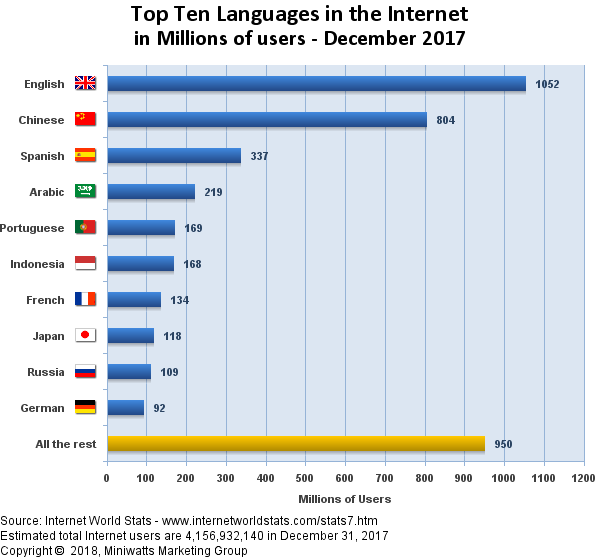
\includegraphics[height=\textheight]{../pics/languages2017Q4.png}

\myslide{On the Internet, nobody knows you are a dog}
\begin{center}
  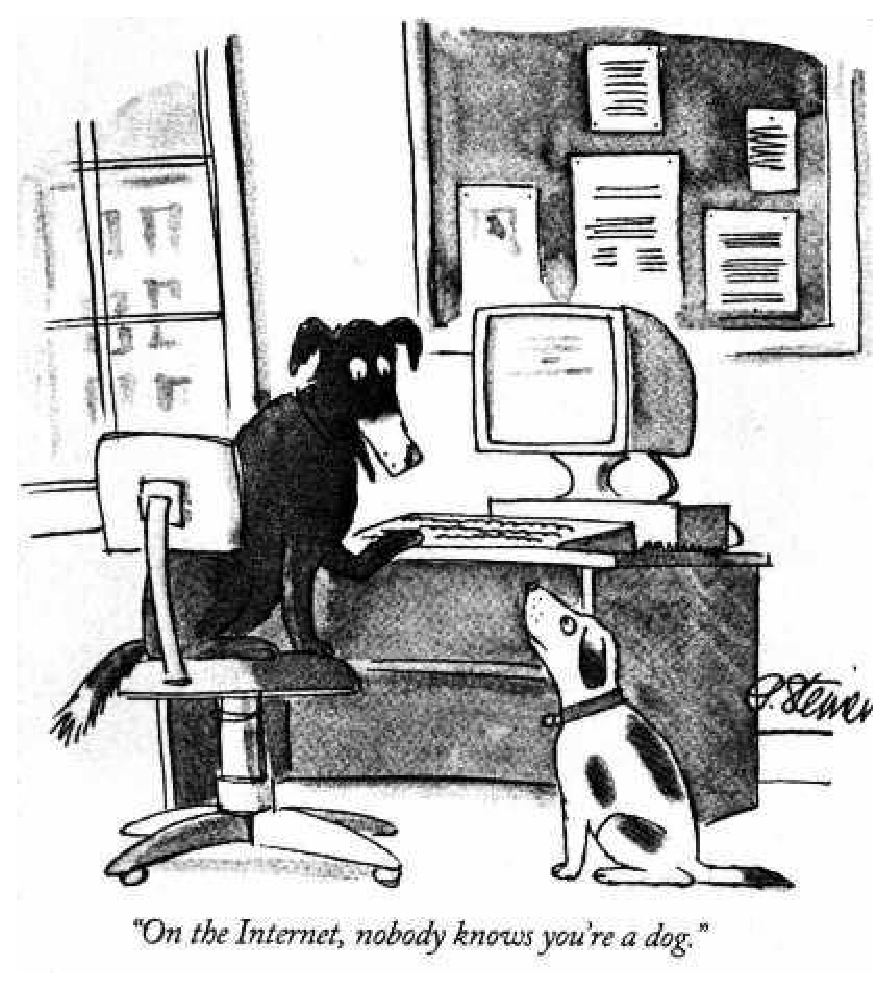
\includegraphics[height=0.9\textheight]{../pics/idog.eps}
\\ Page 61 of July 5, 1993 issue of The New Yorker, (Vol.69 (LXIX) no. 20)
\end{center}
\newpage
\begin{center}
  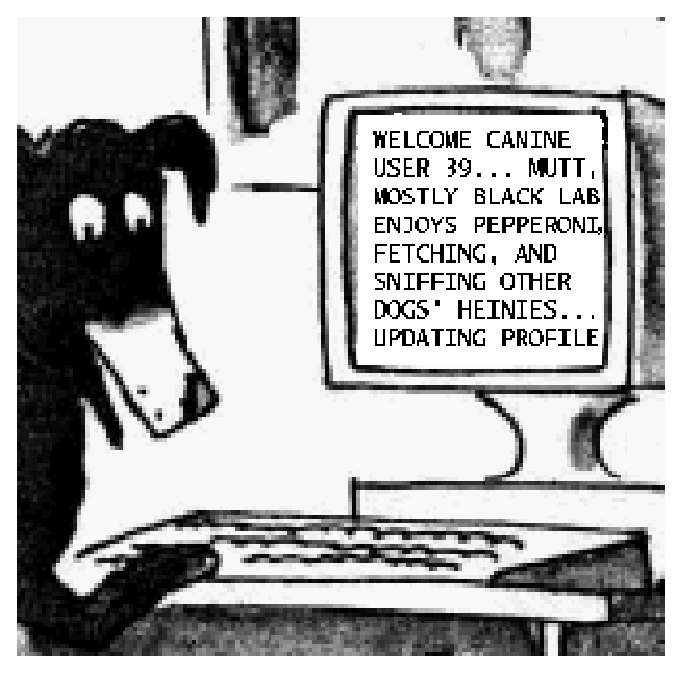
\includegraphics[height=0.8\textheight]{../pics/dog3.eps}
\url{http://www.unc.edu/depts/jomc/academics/dri/idog.html}
\end{center}

% \myslide{What does the web know about us?}

% \begin{itemize}
% \item http://personas.media.mit.edu/personasWeb.html
% \end{itemize}

\myslide{Some Technical Terms (the squiggly bits)}

\myslide{A gentle introduction to Information theory}

\begin{itemize}
\item Language has many uses, only one of which is to convey information
  \\ \textit{A bit of Fry and Laurie Season 1 Episode 2}
  \\ --- but surely transferring information is important
\item How can we measure information?
  \begin{itemize}
  \item Information as Bits
\\ {\small Shannon, C.E. (1948), "A Mathematical Theory of Communication", Bell System Technical Journal, 27, pp. 379–423 \& 623–656, July \& October, 1948. \url{http://cm.bell-labs.com/cm/ms/what/shannonday/shannon1948.pdf}}
  \item Minimum Description Length
\\ {\small Andrey Kolmogorov (1968), "Three approaches to the quantitative definition of information" in International Journal of Computer Mathematics.}
  \end{itemize}
\end{itemize}

\myslide{Consider an abstract case}
\begin{center}
  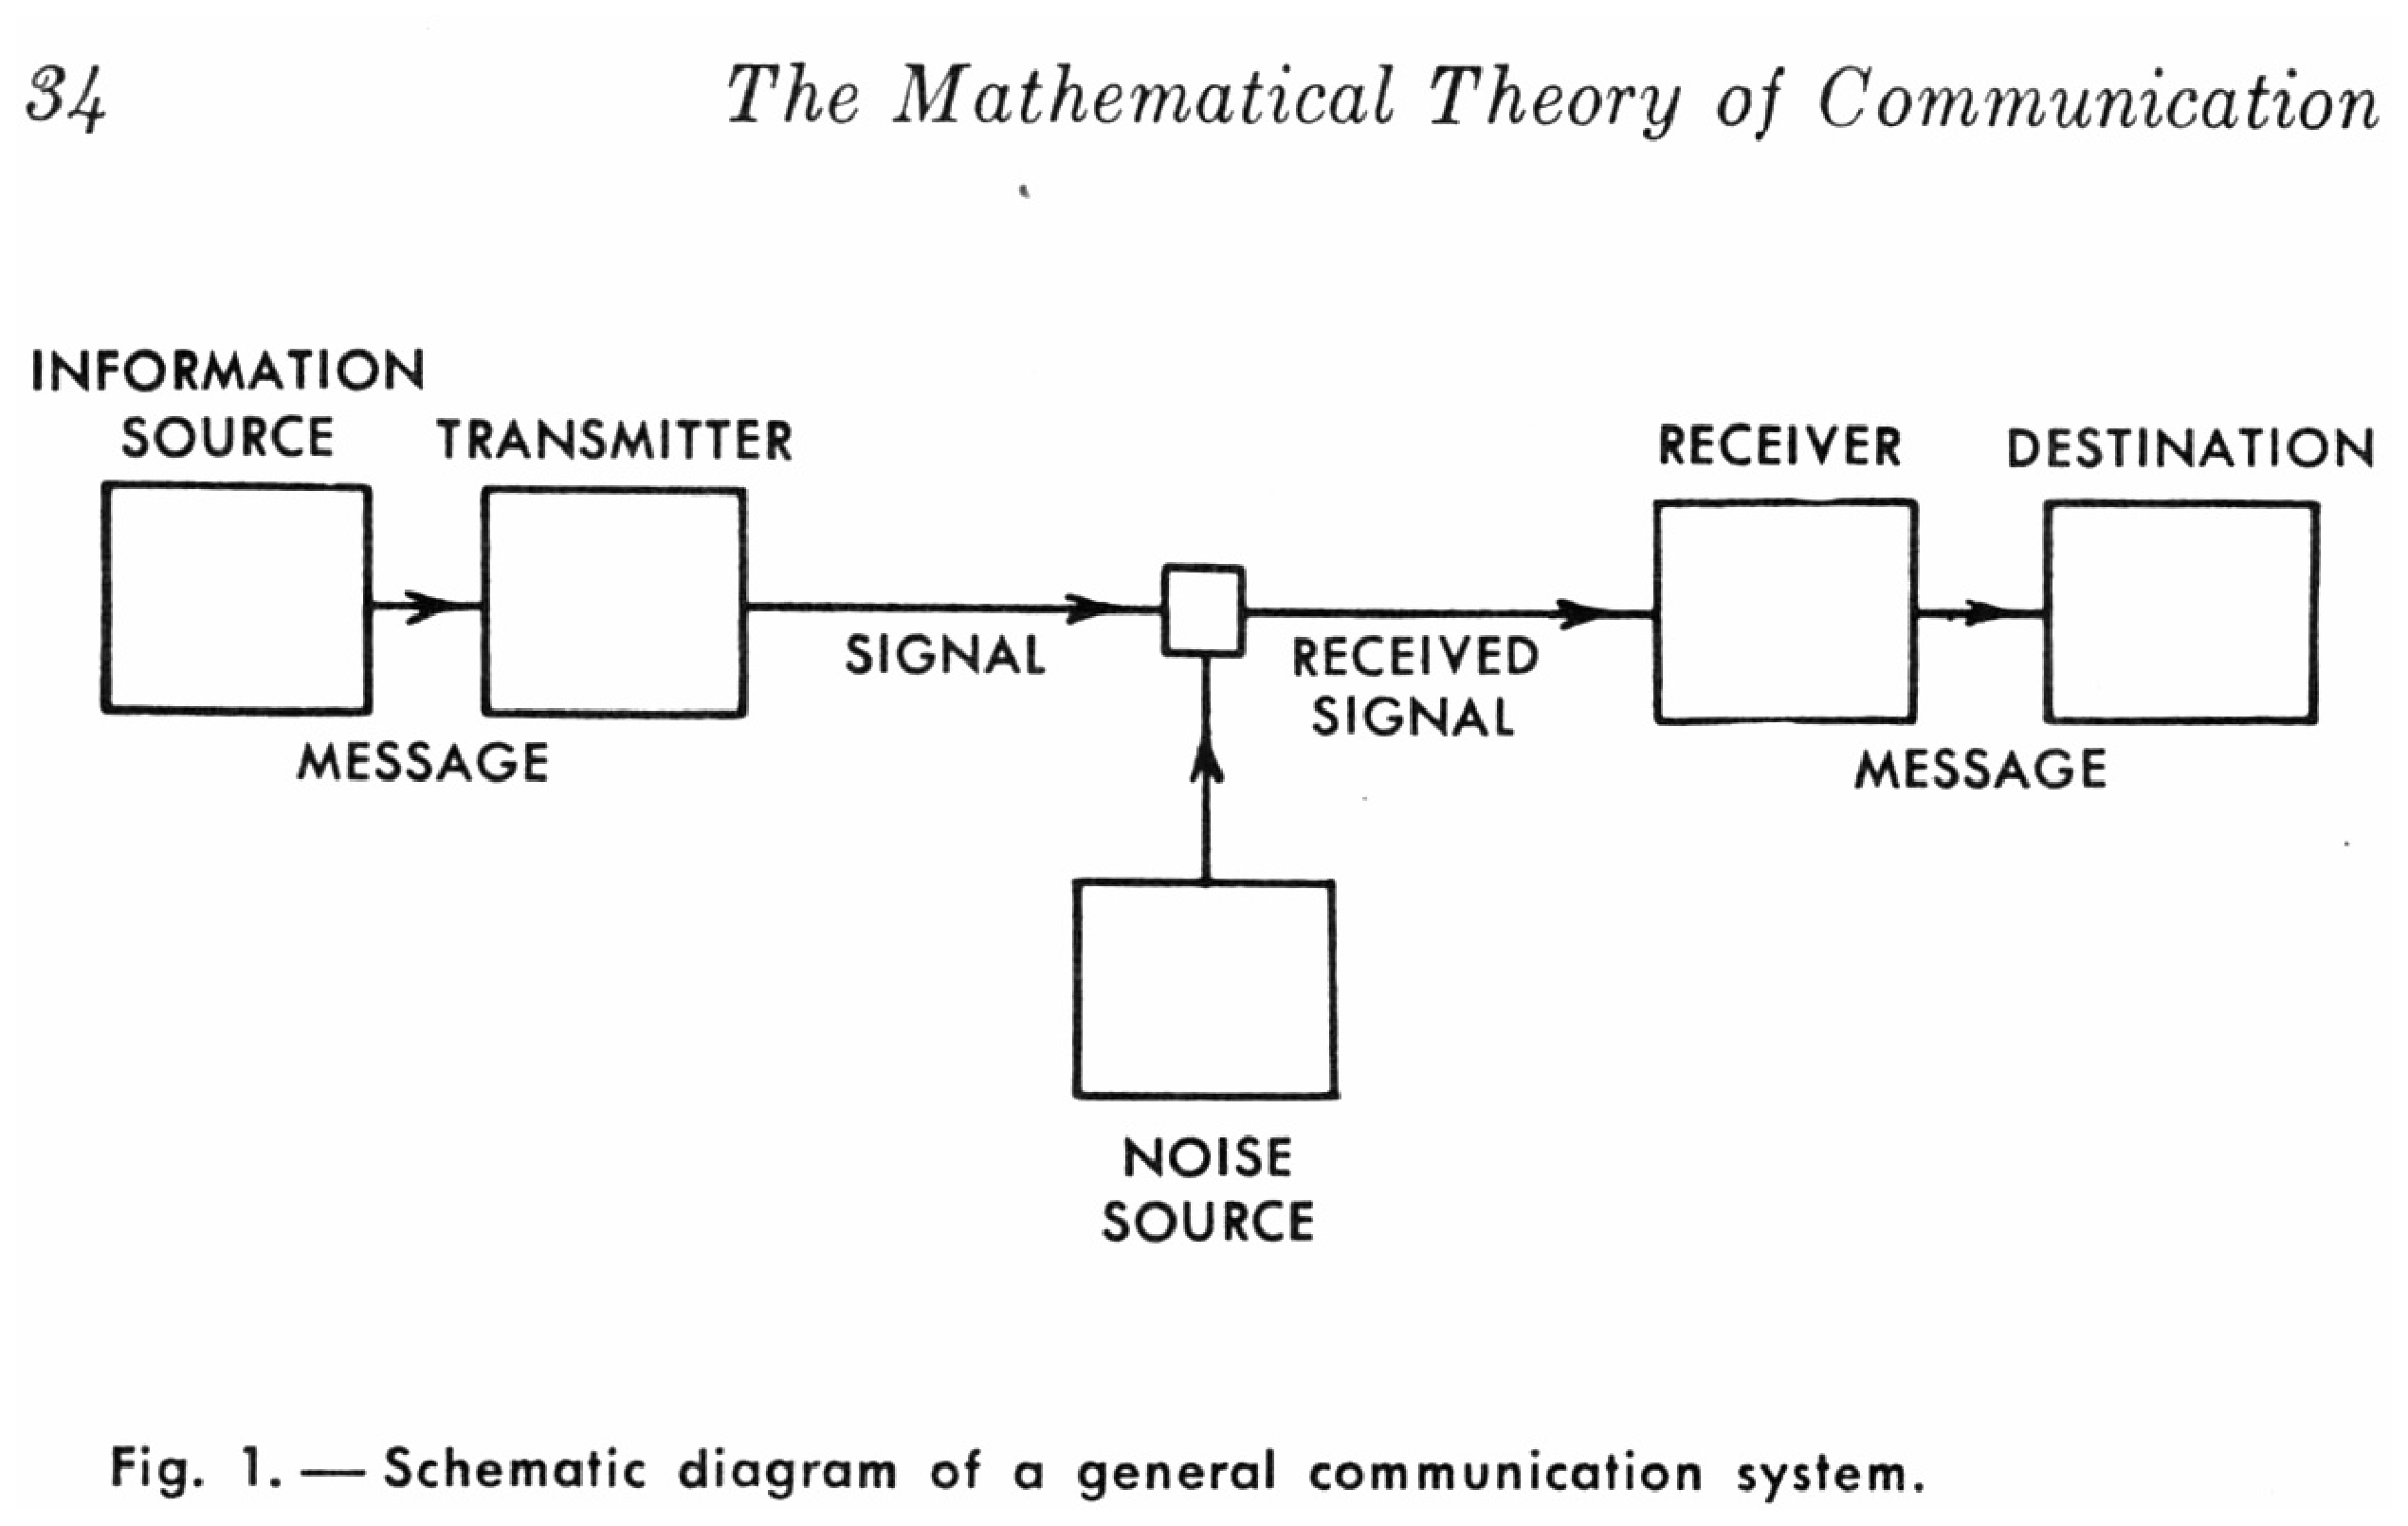
\includegraphics[height=0.9\textheight]{../pics/shannon_comm_channel}
\end{center}


\myslide{Information as bits}

\begin{itemize}
\item Suppose we have 8 equally likely facts (A, B, C, \ldots H). 
 \\ How many yes-no   questions does it take to pinpoint the fact?
  \begin{itemize}
  \item This is the information in bits
\\ you need $n$ bits of information
  \end{itemize}
  \item Technically the Entropy %
 \[ H(\mathrm{p}) = -\sum_{x \in X} \mathrm{p}(x)\log_2\mathrm{p}(x) \]
 %\[ H(\mathrm{p}) = -\sum_{x \in X} \mathrm{p}(x)\log_2\mathrm{p}(x) \]
    \begin{itemize}
    \item  We won't go there in HG2052
    \end{itemize}
  \end{itemize}

\myslide{What if some facts are more common?}

\begin{itemize}
\item Simplified Polynesian:
\\  p ($\frac{1}{8}$);
k ($\frac{1}{8}$);
i ($\frac{1}{8}$);
u ($\frac{1}{8}$);
   t ($\frac{1}{4}$);
   a ($\frac{1}{4}$)
\item We can do this in $2 \frac{1}{2}$ bits
  \begin{itemize}
  \item Is it (a or t) or ( p, k, i, u), \ldots
  \end{itemize}
\item We can define a $2 \frac{1}{2}$ bit code 
  \begin{itemize}
  \item p (100); k (101); i (110); u (111); t (00);  a (01)  
  \end{itemize}
\item Which codes are longer --- frequent or infrequent letters?
  \begin{itemize}
  \item What does this imply for language?
  \end{itemize}
\end{itemize}

\citep[\S2.2]{Manning:Schuetze:1999}


\myslide{What if there is mutual information?}

\begin{itemize}
\item What is the next letter?
\item What is the next letter following /./?
  \begin{itemize}
  \item [t]
  \item [a]
  \item [q]
  \end{itemize}
\item What is the next letter following /../?
  \begin{itemize}
  \item [th]
  \item [as]
  \item [qu]
  \end{itemize}
\item A language model and more context improves our guess
\end{itemize}


\myslide{Different Models for English}

Consider only 26 lowercase letters and a space, and a language model
based on probability (Hidden Markov Model).  How many guesses do we
need on average to guess the next letter?

\begin{itemize}
\item Zeroth order (random) = $\log_2$ 27 = 4.76
\item First order (frequency) = 4.03 \hfill (pick \textit{e})
\item Second order (one previous letter) = 2.8
\item Human = 1.34
\end{itemize}

Surrounding context helps interpretation


\myslide{What if there is noise?}

\begin{itemize}
\item Imagine you want to send a signal, but randomly a bit gets flipped (noise)
  \begin{itemize}
  \item Original message /pa/ 100 01
  \item Received message /ka/ 101 01
  \end{itemize}
\item If we make the message longer, we can guard against this
  \begin{itemize}
  \item Original message /pa/ 100 100 100 01 01 01
  \item Received message /ka/ 101 100 100 01 01 01
\\   We add \blu{redundancy} to the signal
\item There are much better encodings than this (\blu{Hamming codes})
\end{itemize}
\item Hmn lngge s vr rdndnt 
\end{itemize}

\myslide{The cloze test}
\newcommand{\cz}[1]{\hspace*{3em}}

Modern linguistics has been \cz{able} to provide theories and \cz{formalisms}
for the specification of \cz{grammars} that express this mapping \cz{in} a
declarative and transparent \cz{way}. Computational linguistics has
contributed \cz{elaborate} platforms and tools for \cz{grammar} development.

A few large \cz{scale} grammars have been \cz{designed} that exhibit sufficient
\cz{accuracy} and coverage for \cz{real} application tasks. However,\cz{ these}
encouraging developments were \cz{seriously} hampered by a \cz{lack} of methods
for \cz{language} analysis that fulfill \cz{the} minimal requirements in
\cz{efficiency}, robustness, and specificity.

This simply \cz{means} that all \cz{systems} working with \cz{these} grammars have
\cz{been} too slow \cz{and} too brittle \cz{for} real applications. \cz{Furthermore}, they
have \cz{not} been able \cz{to} manage the \cz{vast} ambiguity in \cz{natural} language,
i.e. \cz{they} could not \cz{select} among large \cz{numbers} of linguistically
\cz{correct} analyses.

\myslide{How did we go?}
Modern linguistics has been {able} to provide theories and {formalisms}
for the specification of {grammars} that express this mapping {in} a
declarative and transparent {way}. Computational linguistics has
contributed {elaborate} platforms and tools for {grammar} development.

A few large scale grammars have been designed that exhibit sufficient
accuracy and coverage for real application tasks. However, these
encouraging developments were seriously hampered by a lack of methods
for language analysis that fulfill the minimal requirements in
efficiency, robustness, and specificity.

This simply means that all systems working with these grammars have
been too slow and too brittle for real applications. Furthermore, they
have not been able to manage the vast ambiguity in natural language,
i.e. they could not select among large numbers of linguistically
correct analyses.

\url{http://www.delph-in.net/index.php?page=1}



\myslide{Minimum Description Length}

\begin{itemize}
\item Which message has more information?
  \begin{itemize}
  \item ababababababababababab
  \item lakdsfiuy,mwskfsfdends
  \end{itemize}
\item We can write the first as ``ab 11 times'' half as many letters
\item The \blu{Minimum description length} is the shortest description
  in some fixed description language
  \\ note: MDL includes the algorithm and data
\item The difference between the actual length and the MDL is the redundancy
\item English appears to have more redundancy that Chinese:
  \\ size(English/Chinese):  Text --- 1.49; Compressed --- 1.14
\\ \url{http://158.130.17.5/~myl/languagelog/archives/002379.html}
\end{itemize}

\myslide{DIKW}
\begin{description}
\item \txx{Data} is unprocessed facts and figures without any added interpretation or analysis. "The price of crude oil is \$80 per barrel."
\item \txx{Information} is data that has been interpreted so that it has meaning for the user. "The price of crude oil has risen from \$70 to \$80 per barrel" gives meaning to the data and so is said to be information to someone who tracks oil prices.
\item \txx{Knowledge} is a combination of information, experience and insight that may benefit the individual or the organisation. "When crude oil prices go up by \$10 per barrel, it's likely that petrol prices will rise by 2p per litre" is knowledge.
%http://searchdatamanagement.techtarget.com/feature/Defining-data-information-and-knowledge
\item \txx{Wisdom} ``knowing the right things to do''
\end{description}


% Bandwidth, Compression S/N ratio

% What \% is what
% \url{http://www.webgenrewiki.org/index.php5/Main_Page}

% Internet diary

% Check Steven's intro



%http://www.unc.edu/depts/jomc/academics/dri/idog.html




\myslide{What about you?}


\begin{itemize}
\item name  (I won't remember it, sorry)
% https://www.livescience.com/54612-misnaming-family-siblings-pets.html
\item what you hope to get out of the class
\item languages you speak
\item something else?
\end{itemize}

\myslide{HomeWork: Who uses what? (will you tell?)}

\begin{itemize} \addtolength{\itemsep}{-0.5ex}
\item Telnet, ftp, ssh
\item WWW
\item Wikis
\item Blogs (overlap)
\item Email (from PC, phone, other)
\item Virtual Worlds
\item Facebook, LinkedIn
\item Twitter, Tumbler, \ldots
\item LT: MT, dictation, other
\end{itemize}


\myslide{HomeWork and Readings}

\begin{itemize}
\item Keep a media usage diary for one day (Friday) and add it to the shared spreadsheet

\item Read the following:
  \begin{itemize}
  \item What can search terms tell us?
    \\ \url{https://www.nature.com/articles/nature07634} (use the proxy)
  \item Which is more efficient: Chinese or English:
    \\ \url{http://itre.cis.upenn.edu/~myl/languagelog/archives/002379.html}
  \item Rants about technology through the ages: 
    \\ Vaughan Bell (2010) Don't touch that Dial! \textit{Slate}
    \\ \url{http://www.slate.com/id/2244198/} accessed 2010-09-03. 
  \end{itemize}
  
\end{itemize}

%Measuring Linguistic Diversity on the Internet
%http://unesdoc.unesco.org/images/0014/001421/142186e.pdf

%%
%% Future
%%

\end{document}

 
%%% Local Variables: 
%%% coding: utf-8
%%% mode: latex
%%% TeX-PDF-mode: t
%%% TeX-engine: xetex
%%% End: 